\documentclass[a4paper,10pt]{report}

\usepackage{epsfig,dsfont}

\newcommand{\ol}[1]{\overline{#1}}
\newcommand{\h}[1]{\hat{#1}}
\newcommand{\rrb}{\overline{\rho}}
\newcommand{\rr}{\rho}
\newcommand{\emu}{e^{\mu}}
\newcommand{\emmu}{e^{-\mu}}
\newcommand{\Mb}{\ol{M}}
\newcommand{\mv}[1]{\langle #1 \rangle}
\newcommand{\pij}[2]{\ol{\psi}_{#1} \psi_{#2}}
\newcommand{\ppb}{\ol{\psi}\psi}
\newcommand{\D}{D^{-1}}

\begin{document}

\begin{center}
{\bf \Large Improved Taylor Expansion for Wilson Fermions} 
\end{center}

\vspace*{10mm}

\noindent The Wilson Dirac operator with chemical potential can be written as

$$
D_{ij}[U](\mu) = (m+4)\delta_{ij} - \sum_{\nu=1}^4 \left( U_\nu(i) \frac{1-\gamma_\nu}{2}\delta_{i+\h{\nu},j} \right.
\left. + U^\dagger_\nu(i-\h{\nu})\frac{1+\gamma_\nu}{2}\delta_{i-\h{\nu},j} \right) - \rr M_{ij} - \rrb \Mb_{ij}
$$

\noindent The parameters $\rr$ and $\rrb$ (that will be used later as expansion
parameters) and the matrices $M$ and $\Mb$
can be defined in two different ways:

\begin{itemize}
\item {\bf Expansion 1}
$$\rr = \emu - 1 \; ;  \rrb = \emmu - 1 \ .$$

\noindent The matrices $M$ and $\Mb$ are:
$$M_{ij} = U_4(i) \frac{1-\gamma_4}{2}\delta_{i+\h{4},j}$$
$$\Mb_{ij} = U_4^\dagger(i-\h{4}) \frac{1+\gamma_4}{2}\delta_{i-\h{4},j}$$

\item {\bf Expansion 2}
$$\rr = e^{N_T\mu} - 1 \; ; \rrb = e^{-N_T\mu} - 1 \ .$$

\noindent The matrices $M$ and $\Mb$ are:
$$M_{ij} = \frac{1-\gamma_4}{2}\delta_{\ol{i},\ol{j}}\delta_{i_4,N_T}\delta_{j_4,1}$$
$$\Mb_{ij} = \frac{1+\gamma_4}{2}\delta_{\ol{i},\ol{j}}\delta_{i_4,1}\delta_{j_4,N_T}$$

\end{itemize}

\noindent The partition sum is
\begin{equation}
 Z(\mu) = \int D[\psi,\ol{\psi},U] e^{-S_G - S_F + R}
\end{equation}
\noindent where $S_G$ is the usual Wilson plaquette action, $S_F$ is the fermionic
action and the quantity $R$ is defined as $\rr \ol{\psi}M\psi + \rrb \ol{\psi}\Mb \psi$.

\vspace*{2mm}
\noindent $e^R$ is complex and cannot be used as part of the probability weights.  
However, it is possible to perform a Taylor expansion of the exponential
for small values of $\rr$ and $\rrb$ and compute all expectation values at zero
chemical potential.  We obtain the following expresion for the partition sum
(up to fourth order or quantities with four propagators):

\begin{equation}
Z(\mu) \approx Z(0)\left[ 1 + \mv{R} + \frac{1}{2} \mv{R^2} + \frac{1}{6} \mv{R^3} + \frac{1}{24} \mv{R^4} \right]
\end{equation}

\noindent To compute the observables we need the logarithm of the partition
sum.  Therefore, we also expand the logarithm up to fourth order (in $R$ or/and number of propagators)
\begin{eqnarray}
\ln Z(\mu) \approx \ln Z(0) + \mv{R} + \frac{1}{2}\mv{R^2} - \frac{1}{2}\mv{R}^2 
+ \frac{1}{6}\mv{R^3} - \frac{1}{2}\mv{R}\mv{R^2} + \frac{1}{3}\mv{R}^3 \nonumber \\ 
- \frac{1}{8}\mv{R^2}^2 - \frac{1}{6}\mv{R}\mv{R^3} + \frac{1}{2}\mv{R}^2\mv{R^2} - \frac{1}{4}\mv{R}^4 + \frac{1}{24}\mv{R^4} 
\end{eqnarray}


We will compute the first and second derivatives with respect to the chemical potential
and the mass for the expansions 1 and 2.  In the following I will write down explicitly
the expressions only for the expansion 1.  It is straight forward to get the expressions
for expansion 2 (replace $\rr$ and $\rrb$ and multiply the derivatives of $R$ with respect
to the chemical potential by $N_T$).


\subsection*{Derivatives with respect to $\mu$}
We need the following derivatives:
\begin{eqnarray}
\frac{\partial R}{\partial \mu} &=& \emu \ol{\psi}M\psi - \emmu \ol{\psi}\Mb \psi := D_- \\
\frac{\partial^2 R}{\partial \mu^2} &=& \emu \ol{\psi}M\psi + \emmu \ol{\psi}\Mb \psi := D_+
\end{eqnarray}

\noindent We compute two observables, the particle number $n$
and its susceptibility $\chi_n$.  The particle number up to fourth
order (in number of propagators) is given by:

\begin{eqnarray}
n = \frac{\partial \ln Z}{\partial \mu} &=& \mv{D_-} + \mv{RD_-} - \mv{R}\mv{D_-}
    + \frac{1}{2}\mv{R^2D_-} - \frac{1}{2}\mv{D_-}\mv{R^2} - \mv{R}\mv{RD_-}   \nonumber \\
  & & + \mv{R}^2\mv{D_-}+ \frac{1}{6}\mv{R^3D_-} - \frac{1}{2}\mv{R^2}\mv{RD_-}
    - \frac{1}{6}\mv{D_-}\mv{R^3} - \frac{1}{2}\mv{R}\mv{R^2D_-}  \nonumber \\
  & & + \mv{R}\mv{D_-}\mv{R^2} + \mv{R}^2\mv{RD_-} - \mv{R}^3\mv{D_-}
\end{eqnarray}

\noindent The susceptibility

\begin{eqnarray}
\chi_n = \frac{\partial^2 \ln Z}{\partial \mu^2} &=& 
  \mv{D_+} + \mv{D^2_-} + \mv{RD_+} - \mv{D_-}^2 - \mv{R}\mv{D_+} + \mv{RD^2_-} + \frac{1}{2}\mv{R^2D_+}\nonumber \\
  && - \frac{1}{2}\mv{D_+}\mv{R^2}
     - 2\mv{D_-}\mv{RD_-} - \mv{R}\mv{D^2_-} - \mv{R}\mv{RD_+} + 2 \mv{R}\mv{D_-}^2   \nonumber \\
 && + \mv{R}^2\mv{D_+} + \frac{1}{2}\mv{R^2D_-^2} + \frac{1}{6}\mv{R^3D_+}
    - \mv{RD_-}^2 - \frac{1}{2}\mv{R^2}\mv{D^2_-} - \frac{1}{2}\mv{R^2}\mv{RD_+}   \nonumber \\
 && - \frac{1}{6}\mv{D_+}\mv{R^3} - \mv{D_-}\mv{R^2D_-} - \mv{R}\mv{RD_-^2} 
    - \frac{1}{2}\mv{R}\mv{R^2D_+} + \mv{D_-}^2\mv{R^2}    \nonumber \\
 &&  + \mv{R}\mv{D_+}\mv{R^2} + 4 \mv{R}\mv{D_-}\mv{RD_-} + \mv{R}^2\mv{D_-^2} + \mv{R}^2\mv{RD_+}   \nonumber \\
 &&  - 3 \mv{R}^2\mv{D_-}^2 - \mv{R}^3\mv{D_+}
\end{eqnarray}

\newpage
\subsection*{Derivatives with respect to $m$}

\noindent We need the following derivative
\begin{eqnarray}
\frac{\partial \mv{O}}{\partial m} &=& 
  \frac{\partial}{\partial m} \frac{1}{Z_0} \int D[\psi,\ol{\psi},U]\exp(-S_G - \ol{\psi}_i D_{ij} \psi_j) O \nonumber\\
  &=& \mv{\psi_i \ol{\psi}_i O} -  \mv{\psi_i \ol{\psi}_i}\mv{O}
\end{eqnarray}

\noindent We compute the observables $\partial \ln Z / \partial m$ (defining $\Psi= \psi_i \ol{\psi}_i$)

\begin{eqnarray}
\frac{\partial \ln Z}{\partial m} &=& 
  \mv{\Psi} - \mv{\Psi}\mv{R} + \mv{\Psi R} - \frac{1}{2}\mv{\Psi}\mv{R^2} + \frac{1}{2}\mv{\Psi R^2} 
   + \mv{R}^2\mv{\Psi}  \nonumber\\ 
   && - \mv{R}\mv{\Psi R} - \frac{1}{6}\mv{\Psi}\mv{R^3}  + \frac{1}{6}\mv{\Psi R^3}
  + \mv{R^2}\mv{\Psi}\mv{R} - \frac{1}{2}\mv{R^2}\mv{\Psi R} \nonumber \\
  && - \frac{1}{2}\mv{R}\mv{\Psi R^2}
  - \mv{R^3}\mv{\Psi} + \mv{R}^2\mv{\Psi R}
\end{eqnarray}


\noindent and its susceptibility

\begin{eqnarray}
\frac{\partial^2 \ln Z}{\partial m^2} &=& 
  \mv{\Psi^2} - \mv{\Psi}^2 + 2 \mv{\Psi}^2\mv{R} - \mv{\Psi^2}\mv{R} 
  - 2 \mv{\Psi}\mv{\Psi R} + \mv{\Psi^2 R} \nonumber \\
  && + \mv{\Psi}^2\mv{R^2} - \frac{1}{2}\mv{\Psi^2}\mv{R^2}
  - \mv{\Psi}\mv{\Psi R^2} + \frac{1}{2}\mv{\Psi^2 R^2} - 3 \mv{\Psi}^2\mv{R}^2 \nonumber \\
  &&  + 4 \mv{\Psi}\mv{R}\mv{\Psi R} 
  + \mv{R}^2\mv{\Psi^2} - \mv{\Psi R}^2 - \mv{R}\mv{\Psi^2 R}
\end{eqnarray}

\subsection*{Explicit expressions for each expectation value}
\subsection*{Terms with one propagator}

To compute the observables we need the following expectation values:

\begin{eqnarray}
\mv{R} &=& - \rr \mv{M_{ij} \pij{j}{i}} - \rrb \mv{\Mb_{ij} \pij{j}{i}}\\
\mv{D_-} &=& - \emu \mv{M_{ij} \pij{j}{i}} + \emmu \mv{\ol{M}_{ij} \pij{j}{i}}\\
\mv{D_+} &=& - \emu \mv{M_{ij} \pij{j}{i}} - \emmu \mv{\ol{M}_{ij} \pij{j}{i}}\\
\mv{\Psi} &=& - \mv{\pij{i}{i}}
\end{eqnarray}

\noindent From the Wick theorem
$$\pij{j}{i} = D^{-1}_{ji}$$

\noindent Then
\begin{itemize}
\item[] $\mv{M_{ij} \pij{j}{i}} = Tr[M\D]$
\item[] $\mv{M_{ij} \pij{j}{i}} = Tr[\Mb\D]$
\item[] $\mv{\pij{i}{i}} = -Tr[\D]$
\end{itemize}


\subsection*{Terms with two propagators}

To compute the observables we need the following expectation values:
\begin{eqnarray}
\mv{R^2} &=& \rr^2 \mv{M_{i_1j_1}M_{i_2j_2} \ppb_{j_1i_1j_2i_2}}
           + 2 \rrb \rr \mv{M_{i_1j_1}\Mb_{i_2j_2} \ppb_{j_1i_1j_2i_2}} \nonumber\\
          && + \rrb^2 \mv{\Mb_{i_1j_1}\Mb_{i_2j_2} \ppb_{j_1i_1j_2i_2}}  \\
\nonumber\\
\mv{D^2_-} &=& e^{2\mu} \mv{M_{i_1j_1}M_{i_2j_2} \ppb_{j_1i_1j_2i_2}}
           - 2 \mv{M_{i_1j_1}\Mb_{i_2j_2} \ppb_{j_1i_1j_2i_2}} \nonumber\\
          && + e^{-2\mu} \mv{\Mb_{i_1j_1}\Mb_{i_2j_2} \ppb_{j_1i_1j_2i_2}} \\
\nonumber\\
\mv{D^2_+} &=& e^{2\mu} \mv{M_{i_1j_1}M_{i_2j_2} \ppb_{j_1i_1j_2i_2}}
           + 2 \mv{M_{i_1j_1}\Mb_{i_2j_2} \ppb_{j_1i_1j_2i_2}} \nonumber\\
          && + e^{-2\mu} \mv{\Mb_{i_1j_1}\Mb_{i_2j_2} \ppb_{j_1i_1j_2i_2}} \\
\nonumber\\
\mv{RD_-} &=& \rr\emu \mv{M_{i_1j_1}M_{i_2j_2} \ppb_{j_1i_1j_2i_2}}
           + (\rrb \emu-\rr \emmu)\mv{M_{i_1j_1}\Mb_{i_2j_2}\ppb_{j_1i_1j_2i_2}} \nonumber\\
          && - \rrb\emmu \mv{\Mb_{i_1j_1}\Mb_{i_2j_2} \ppb_{j_1i_1j_2i_2}} \\
\nonumber\\
\mv{RD_+} &=& \rr\emu \mv{M_{i_1j_1}M_{i_2j_2} \ppb_{j_1i_1j_2i_2}}
          + (\rr \emmu + \rrb \emu)\mv{M_{i_1j_1}\Mb_{i_2j_2} \ppb_{j_1i_1j_2i_2}} \nonumber\\
          && + \rrb\emmu \mv{\Mb_{i_1j_1}\Mb_{i_2j_2} \ppb_{j_1i_1j_2i_2}} \\
\nonumber\\
\mv{\Psi^2} &=& \mv{\ppb_{i_1i_1i_2i_2}} \\
\nonumber\\
\mv{\Psi R} &=&  - \rr \mv{M_{i_2j_2}\ppb_{i_1i_1j_2i_2}} - \rrb \mv{\Mb_{i_2j_2} \ppb_{i_1i_1j_2i_2}}
\end{eqnarray}


\noindent From the Wick theorem
$$\ppb_{j_1i_1j_2i_2} = \D_{j_1i_1}\D_{j_2i_2} - \D_{j_1i_2}\D_{j_2i_1}$$

\noindent Then
\begin{itemize}
\item[] $\mv{M_{i_1j_1}M_{i_2j_2} \ppb_{j_1i_1j_2i_2}} = Tr[M\D]^2 - Tr[M\D M\D]$
\item[] $\mv{M_{i_1j_1}\Mb_{i_2j_2} \ppb_{j_1i_1j_2i_2}} = Tr[M\D]Tr[\Mb\D] - Tr[M\D \Mb\D]$
\item[] $\mv{\Mb_{i_1j_1}\Mb_{i_2j_2} \ppb_{j_1i_1j_2i_2}} = Tr[\Mb\D]^2 - Tr[\Mb\D \Mb\D]$

\item[] $\mv{M_{i_2j_2} \ppb_{i_1i_1j_2i_2}} = Tr[\D]Tr[M\D] - Tr[\D M \D]$
\item[] $\mv{\Mb_{i_2j_2} \ppb_{i_1i_1j_2i_2}} = Tr[\D]Tr[\Mb\D] - Tr[\D \Mb \D]$
\item[] $\mv{\ppb_{i_1i_1i_2i_2}} = Tr[\D]^2 - Tr[\D\D]$
\end{itemize}

\newpage
\subsection*{Terms with three propagators}

To compute the observables we need the following expectation values:
\begin{eqnarray}
\mv{R^3} &=& -\rr^3  \mv{M_{i_1j_1}M_{i_2j_2}M_{i_3j_3} \ppb_{j_1i_1...j_3i_3}}
           -  \rrb^3 \mv{\Mb_{i_1j_1}\Mb_{i_2j_2}\Mb_{i_3j_3} \ppb_{j_1i_1...j_3i_3}} \nonumber\\
          && - 3 \rr^2\rrb \mv{M_{i_1j_1}M_{i_2j_2}\Mb_{i_3j_3} \ppb_{j_1i_1...j_3i_3}} \nonumber\\
          && - 3 \rrb^2\rr \mv{M_{i_1j_1}\Mb_{i_2j_2}\Mb_{i_3j_3} \ppb_{j_1i_1...j_3i_3}}    \\
\nonumber\\
\mv{R^2D_-} &=& -\rr^2\emu  \mv{M_{i_1j_1}M_{i_2j_2}M_{i_3j_3} \ppb_{j_1i_1...j_3i_3}}\nonumber\\
          && +  \rrb^2\emmu \mv{\Mb_{i_1j_1}\Mb_{i_2j_2}\Mb_{i_3j_3} \ppb_{j_1i_1...j_3i_3}} \nonumber\\
          && + (\emmu\rr^2 - 2 \rr\rrb\emu) \mv{M_{i_1j_1}M_{i_2j_2}\Mb_{i_3j_3} \ppb_{j_1i_1...j_3i_3}} \nonumber\\
          && + (-\emu\rrb^2 + 2 \rr\rrb\emmu) \mv{M_{i_1j_1}\Mb_{i_2j_2}\Mb_{i_3j_3} \ppb_{j_1i_1...j_3i_3}}    \\
\nonumber\\
\mv{R^2D_+} &=& -\rr^2\emu  \mv{M_{i_1j_1}M_{i_2j_2}M_{i_3j_3} \ppb_{j_1i_1...j_3i_3}}\nonumber\\
          && -  \rrb^2\emmu \mv{\Mb_{i_1j_1}\Mb_{i_2j_2}\Mb_{i_3j_3} \ppb_{j_1i_1...j_3i_3}} \nonumber\\
          && - (\emmu\rr^2 + 2 \rr\rrb\emu) \mv{M_{i_1j_1}M_{i_2j_2}\Mb_{i_3j_3} \ppb_{j_1i_1...j_3i_3}} \nonumber\\
          && - (\emu\rrb^2 + 2 \rr\rrb\emmu) \mv{M_{i_1j_1}\Mb_{i_2j_2}\Mb_{i_3j_3} \ppb_{j_1i_1...j_3i_3}} \\
\nonumber\\
\mv{RD_-^2} &=& -\rr e^{2\mu}  \mv{M_{i_1j_1}M_{i_2j_2}M_{i_3j_3} \ppb_{j_1i_1...j_3i_3}}\nonumber\\
          && -  \rrb e^{-2\mu} \mv{\Mb_{i_1j_1}\Mb_{i_2j_2}\Mb_{i_3j_3} \ppb_{j_1i_1...j_3i_3}} \nonumber\\
          && + (2\rr-\rrb e^{2\mu}) \mv{M_{i_1j_1}M_{i_2j_2}\Mb_{i_3j_3} \ppb_{j_1i_1...j_3i_3}} \nonumber\\
          && + (2\rrb-\rr e^{-2\mu}) \mv{M_{i_1j_1}\Mb_{i_2j_2}\Mb_{i_3j_3} \ppb_{j_1i_1...j_3i_3}}    \\
\nonumber\\
\mv{\Psi R^2} &=& \rr^2 \mv{M_{i_1j_1}M_{i_2j_2} \ppb_{j_1i_1...i_3i_3}} \nonumber\\
          && +  \rrb \rr \mv{M_{i_1j_1}\Mb_{i_2j_2} \ppb_{j_1i_1...i_3i_3}} 
          + \rrb \rr \mv{\Mb_{i_1j_1}M_{i_2j_2} \ppb_{j_1i_1...i_3i_3}} \nonumber\\
          && + \rrb^2 \mv{\Mb_{i_1j_1}\Mb_{i_2j_2}\ppb_{j_1i_1...i_3i_3}}    \\
\nonumber\\
\mv{\Psi^2 R} &=&  - \rr \mv{M_{i_1j_1}\ppb_{j_1i_1...i_3i_3}} - \rrb \mv{\Mb_{i_1j_1} \ppb_{j_1i_1...i_3i_3}}
\end{eqnarray}

\vspace*{3mm}
\noindent From the Wick theorem
\begin{eqnarray}
\ppb_{j_1i_1...j_3i_3} &=& \D_{j_1i_1}\D_{j_2i_2}\D_{j_3i_3} + \D_{j_1i_2}\D_{j_2i_3}\D_{j_3i_1} 
		   + \D_{j_1i_3}\D_{j_2i_1}\D_{j_3i_2} \nonumber\\&& - \D_{j_1i_3}\D_{j_2i_2}\D_{j_3i_1}
		   - \D_{j_1i_1}\D_{j_2i_3}\D_{j_3i_2}- \D_{j_1i_2}\D_{j_2i_1}\D_{j_3i_3} \nonumber
\end{eqnarray}

\newpage
\noindent Then
\begin{eqnarray}
\mv{M_{i_1j_1}M_{i_2j_2}M_{i_3j_3} \ppb_{j_1i_1...j_3i_3}} &=& 
Tr[M\D]^3 - 3 Tr[M\D]Tr[(M\D)^2] + 2Tr[(M\D)^3] \nonumber\\
\nonumber\\
\mv{M_{i_1j_1}M_{i_2j_2}\Mb_{i_3j_3} \ppb_{j_1i_1...j_3i_3}} &=& 
Tr[M\D]^2Tr[\Mb\D] - Tr[\Mb\D]Tr[(M\D)^2] \nonumber \\
&& - 2 Tr[M\D]Tr[M\D \Mb\D] +  2Tr[\Mb\D(M\D)^2] \nonumber\\
\nonumber\\
\mv{M_{i_1j_1}\Mb_{i_2j_2}\Mb_{i_3j_3} \ppb_{j_1i_1...j_3i_3}} &=& 
Tr[\Mb\D]^2Tr[M\D] - Tr[M\D]Tr[(\Mb\D)^2] \nonumber \\
&& - 2 Tr[\Mb\D]Tr[M\D \Mb\D] +  2Tr[M\D(\Mb\D)^2] \nonumber\\
\nonumber\\
\mv{\Mb_{i_1j_1}\Mb_{i_2j_2}\Mb_{i_3j_3} \ppb_{j_1i_1...j_3i_3}} &=& 
Tr[\Mb\D]^3 - 3 Tr[\Mb\D]Tr[(\Mb\D)^2] + 2Tr[(\Mb\D)^3] \nonumber\\
\nonumber\\
%
\mv{M_{i_1j_1}M_{i_2j_2} \ppb_{j_1i_1...i_3i_3}} &=& 
Tr[M\D]^2Tr[\D] - Tr[\D]Tr[(M\D)^2] \nonumber \\
&& - 2 Tr[M\D]Tr[\D M\D] +  2Tr[\D(M\D)^2] \nonumber\\
\nonumber\\
\mv{M_{i_1j_1}\Mb_{i_2j_2} \ppb_{j_1i_1...i_3i_3}} &=& 
Tr[\D]Tr[M\D]Tr[\Mb\D] - Tr[\D]Tr[M\D \Mb \D] \nonumber \\
&& - Tr[M \D]Tr[\D\Mb\D] - Tr[\Mb\D]Tr[\D M \D] \nonumber\\
&& +  2Tr[\D M\D\Mb\D] \nonumber\\
\nonumber\\
\mv{\Mb_{i_1j_1}M_{i_2j_2} \ppb_{j_1i_1...i_3i_3}} &=& 
Tr[\D]Tr[M\D]Tr[\Mb\D] - Tr[\D]Tr[M\D \Mb \D] \nonumber \\
&& - Tr[M \D]Tr[\D\Mb\D] - Tr[\Mb\D]Tr[\D M \D]\nonumber\\
&& +  2Tr[\D\Mb\D M\D] \nonumber\\
\nonumber\\
\mv{\Mb_{i_1j_1}\Mb_{i_2j_2} \ppb_{j_1i_1...i_3i_3}} &=& 
Tr[\Mb\D]^2Tr[\D] - Tr[\D]Tr[(\Mb\D)^2] \nonumber \\
&& - 2 Tr[\Mb\D]Tr[\D \Mb\D] +  2Tr[\D(\Mb\D)^2] \nonumber\\
%
\nonumber\\
\mv{M_{i_1j_1} \ppb_{j_1i_1...i_3i_3}} &=& 
Tr[M\D]Tr[\D]^2 - Tr[M\D]Tr[\D\D] \nonumber \\
&& - 2 Tr[\D]Tr[\D M\D] +  2Tr[\D M\D\D] \nonumber\\
\nonumber\\
\mv{\Mb_{i_1j_1} \ppb_{j_1i_1...i_3i_3}} &=& 
Tr[\Mb\D]Tr[\D]^2 - Tr[\Mb\D]Tr[\D\D] \nonumber \\
&& - 2 Tr[\D]Tr[\D \Mb\D] +  2Tr[\D\Mb\D\D] \nonumber
\end{eqnarray}

\newpage
\subsection*{Terms with four propagators}

To compute the observables we need the following expectation values:
\begin{eqnarray}
\mv{R^3D_-} &=& \rr^3\emu  \mv{M_{i_1j_1}M_{i_2j_2}M_{i_3j_3}M_{i_4j_4} \ppb_{j_1i_1...j_4i_4}}\nonumber\\
          && + (3\rrb\rr^2\emu - \rr^3\emmu) \mv{M_{i_1j_1}M_{i_2j_2}M_{i_3j_3}\Mb_{i_4j_4} \ppb_{j_1i_1...j_4i_4}} \nonumber\\
          && + 2(\rr\rrb^2\emu - \rrb\rr^2\emmu) \mv{M_{i_1j_1}M_{i_2j_2}\Mb_{i_3j_3}\Mb_{i_4j_4} \ppb_{j_1i_1...j_4i_4}} \nonumber\\
          && + (\rr\rrb^2\emu - \rrb\rr^2\emmu) \mv{M_{i_1j_1}\Mb_{i_2j_2}M_{i_3j_3}\Mb_{i_4j_4} \ppb_{j_1i_1...j_4i_4}} \nonumber\\
          && + (\rrb^3\emu - 3\rr\rrb^2\emmu) \mv{M_{i_1j_1}\Mb_{i_2j_2}\Mb_{i_3j_3}\Mb_{i_4j_4} \ppb_{j_1i_1...j_4i_4}} \nonumber\\
          && - \rrb^3\emmu \mv{\Mb_{i_1j_1}\Mb_{i_2j_2}\Mb_{i_3j_3}\Mb_{i_4j_4} \ppb_{j_1i_1...j_4i_4}}    \\
\nonumber\\
\mv{R^3D_+} &=& \rr^3\emu  \mv{M_{i_1j_1}M_{i_2j_2}M_{i_3j_3}M_{i_4j_4} \ppb_{j_1i_1...j_4i_4}}\nonumber\\
          && + (3\rrb\rr^2\emu + \rr^3\emmu) \mv{M_{i_1j_1}M_{i_2j_2}M_{i_3j_3}\Mb_{i_4j_4} \ppb_{j_1i_1...j_4i_4}} \nonumber\\
          && + 2(\rr\rrb^2\emu + \rrb\rr^2\emmu) \mv{M_{i_1j_1}M_{i_2j_2}\Mb_{i_3j_3}\Mb_{i_4j_4} \ppb_{j_1i_1...j_4i_4}} \nonumber\\
          && + (\rr\rrb^2\emu + \rrb\rr^2\emmu) \mv{M_{i_1j_1}\Mb_{i_2j_2}M_{i_3j_3}\Mb_{i_4j_4} \ppb_{j_1i_1...j_4i_4}} \nonumber\\
          && + (\rrb^3\emu + 3\rr\rrb^2\emmu) \mv{M_{i_1j_1}\Mb_{i_2j_2}\Mb_{i_3j_3}\Mb_{i_4j_4} \ppb_{j_1i_1...j_4i_4}} \nonumber\\
          && + \rrb^3\emmu \mv{\Mb_{i_1j_1}\Mb_{i_2j_2}\Mb_{i_3j_3}\Mb_{i_4j_4} \ppb_{j_1i_1...j_4i_4}}    \\
\nonumber\\
\mv{R^2D^2_-} &=& \rr^2e^{2\mu}  \mv{M_{i_1j_1}M_{i_2j_2}M_{i_3j_3}M_{i_4j_4} \ppb_{j_1i_1...j_4i_4}}\nonumber\\
          && + 2(\rrb\rr e^{2\mu} - \rr^2) \mv{M_{i_1j_1}M_{i_2j_2}M_{i_3j_3}\Mb_{i_4j_4} \ppb_{j_1i_1...j_4i_4}} \nonumber\\
          && + (\rr^2e^{-2\mu} + \rrb^2e^{2\mu} - 2\rr\rrb) \mv{M_{i_1j_1}M_{i_2j_2}\Mb_{i_3j_3}\Mb_{i_4j_4} \ppb_{j_1i_1...j_4i_4}} \nonumber\\
          && - 2 \rr\rrb \mv{M_{i_1j_1}\Mb_{i_2j_2}M_{i_3j_3}\Mb_{i_4j_4} \ppb_{j_1i_1...j_4i_4}} \nonumber\\
          && + 2(\rr\rrb e^{-2\mu} - \rrb^2) \mv{M_{i_1j_1}\Mb_{i_2j_2}\Mb_{i_3j_3}\Mb_{i_4j_4} \ppb_{j_1i_1...j_4i_4}} \nonumber\\
          && + \rrb^2e^{-2\mu} \mv{\Mb_{i_1j_1}\Mb_{i_2j_2}\Mb_{i_3j_3}\Mb_{i_4j_4} \ppb_{j_1i_1...j_4i_4}}    \\
\nonumber\\
\mv{\Psi^2R^2} &=& \rr^2  \mv{M_{i_1j_1}M_{i_2j_2} \ppb_{j_1i_1...i_4i_4}}
           + \rrb\rr \mv{M_{i_1j_1}\Mb_{i_2j_2} \ppb_{j_1i_1...i_4i_4}} \nonumber\\
          && + \rr\rrb \mv{\Mb_{i_1j_1}M_{i_2j_2} \ppb_{j_1i_1...i_4i_4}}
           + \rrb^2  \mv{\Mb_{i_1j_1}\Mb_{i_2j_2} \ppb_{j_1i_1...i_4i_4}}    \\
\nonumber\\
\mv{\Psi R^3} &=& -\rr^3  \mv{M_{i_1j_1}M_{i_2j_2}M_{i_3j_3} \ppb_{j_1i_1...i_4i_4}}
             - \rr^2\rrb \mv{M_{i_1j_1}M_{i_2j_2}\Mb_{i_3j_3} \ppb_{j_1i_1...i_4i_4}} \nonumber\\
          && - \rr^2\rrb \mv{M_{i_1j_1}\Mb_{i_2j_2}M_{i_3j_3} \ppb_{j_1i_1...i_4i_4}} 
           - \rr^2\rrb \mv{\Mb_{i_1j_1}M_{i_2j_2}M_{i_3j_3} \ppb_{j_1i_1...i_4i_4}} \nonumber\\
          && - \rrb^2\rr \mv{M_{i_1j_1}\Mb_{i_2j_2}\Mb_{i_3j_3} \ppb_{j_1i_1...i_4i_4}}
           - \rrb^2\rr \mv{\Mb_{i_1j_1}M_{i_2j_2}\Mb_{i_3j_3} \ppb_{j_1i_1...i_4i_4}} \nonumber\\
          && - \rrb^2\rr \mv{\Mb_{i_1j_1}\Mb_{i_2j_2}M_{i_3j_3} \ppb_{j_1i_1...i_4i_4}} 
           - \rrb^3 \mv{\Mb_{i_1j_1}\Mb_{i_2j_2}\Mb_{i_3j_3} \ppb_{j_1i_1...i_4i_4}}\nonumber\\
\end{eqnarray}

\noindent From the Wick theorem
\begin{eqnarray}
\ppb_{j_1i_1...j_4i_4} &=& \D_{j_1i_1}\D_{j_2i_2}\D_{j_3i_3}\D_{j_4i_4}
			 +  \D_{j_1i_1}\D_{j_2i_3}\D_{j_3i_4}\D_{j_4i_2}
			 +  \D_{j_1i_1}\D_{j_2i_4}\D_{j_3i_2}\D_{j_4i_3}\nonumber\\
		&&	 +  \D_{j_1i_3}\D_{j_2i_2}\D_{j_3i_4}\D_{j_4i_1}
			 +  \D_{j_1i_4}\D_{j_2i_2}\D_{j_3i_1}\D_{j_4i_3}
			 +  \D_{j_1i_2}\D_{j_2i_4}\D_{j_3i_3}\D_{j_4i_1}\nonumber\\
		&&	 +  \D_{j_1i_4}\D_{j_2i_1}\D_{j_3i_3}\D_{j_4i_2}
			 +  \D_{j_1i_2}\D_{j_2i_3}\D_{j_3i_1}\D_{j_4i_4}
			 +  \D_{j_1i_3}\D_{j_2i_1}\D_{j_3i_2}\D_{j_4i_4}\nonumber\\
		&&	 -  \D_{j_1i_1}\D_{j_2i_2}\D_{j_3i_4}\D_{j_4i_3}
			 -  \D_{j_1i_1}\D_{j_2i_4}\D_{j_3i_3}\D_{j_4i_2}
			 -  \D_{j_1i_1}\D_{j_2i_3}\D_{j_3i_2}\D_{j_4i_4}\nonumber\\	 
		&&	 -  \D_{j_1i_4}\D_{j_2i_2}\D_{j_3i_3}\D_{j_4i_1}
			 -  \D_{j_1i_3}\D_{j_2i_2}\D_{j_3i_1}\D_{j_4i_4}
			 -  \D_{j_1i_2}\D_{j_2i_1}\D_{j_3i_3}\D_{j_4i_4}\nonumber\\
		&&	 +  \D_{j_1i_2}\D_{j_2i_1}\D_{j_3i_4}\D_{j_4i_3}
			 +  \D_{j_1i_3}\D_{j_2i_4}\D_{j_3i_1}\D_{j_4i_2}
			 +  \D_{j_1i_4}\D_{j_2i_3}\D_{j_3i_2}\D_{j_4i_1}\nonumber\\
		&&	 -  \D_{j_1i_2}\D_{j_2i_3}\D_{j_3i_4}\D_{j_4i_1}
			 -  \D_{j_1i_2}\D_{j_2i_4}\D_{j_3i_1}\D_{j_4i_3}
			 -  \D_{j_1i_3}\D_{j_2i_1}\D_{j_3i_4}\D_{j_4i_2}\nonumber\\
		&&	 -  \D_{j_1i_3}\D_{j_2i_4}\D_{j_3i_2}\D_{j_4i_1}
			 -  \D_{j_1i_4}\D_{j_2i_3}\D_{j_3i_1}\D_{j_4i_2}
			 -  \D_{j_1i_4}\D_{j_2i_1}\D_{j_3i_2}\D_{j_4i_3}\nonumber
\end{eqnarray}

\hspace*{-15mm}\noindent Then
\begin{eqnarray}
\hspace*{-19mm}\mv{M_{i_1j_1}M_{i_2j_2}M_{i_3j_3}M_{i_4j_4} \ppb_{j_1i_1...j_4i_4}} &=& 
Tr[M\D]^4 - 6 Tr[M\D]^2Tr[(M\D)^2]  \nonumber\\
&& + 3 Tr[(M\D)^2]^2 + 8 Tr[M\D]Tr[(M\D)^3] - 6 Tr[(M\D)^4]\nonumber\\
\nonumber\\
\hspace*{-19mm}\mv{M_{i_1j_1}M_{i_2j_2}M_{i_3j_3}\Mb_{i_4j_4} \ppb_{j_1i_1...j_4i_4}} &=&
Tr[M\D]^3 Tr[\Mb\D] - 3 Tr[\Mb\D]Tr[M\D]Tr[(M\D)^2] \nonumber\\
&& - 3 Tr[M\D]^2Tr[M\D\Mb\D] + 3 Tr[M\D\Mb\D]Tr[(M\D)^2] \nonumber\\
&&+ 2 Tr[\Mb\D]Tr[(M\D)^3]+ 6 Tr[M\D]Tr[(M\D)^2\Mb\D]\nonumber\\
&&  - 6 Tr[(M\D)^3\Mb\D]\nonumber\\
\nonumber\\
\hspace*{-19mm}\mv{M_{i_1j_1}M_{i_2j_2}\Mb_{i_3j_3}\Mb_{i_4j_4} \ppb_{j_1i_1...j_4i_4}} &=&
Tr[M\D]^2 Tr[\Mb\D]^2 - Tr[\Mb\D]^2Tr[(M\D)^2]\nonumber\\
&& - 4 Tr[M\D]Tr[\Mb\D]Tr[M\D\Mb\D] - Tr[M\D]^2Tr[(\Mb\D)^2] \nonumber\\
&& + Tr[(\Mb\D)^2]Tr[(M\D)^2] + 2 Tr[M\D\Mb\D]^2 \nonumber \\
&& + 4 Tr[M\D]Tr[M\D(\Mb\D)^2] + 4 Tr[\Mb\D]Tr[\Mb\D(M\D)^2] \nonumber\\
&& - 6 Tr[(M\D)^2(\Mb\D)^2]\nonumber\\
\nonumber\\
\hspace*{-19mm}\mv{M_{i_1j_1}\Mb_{i_2j_2}M_{i_3j_3}\Mb_{i_4j_4} \ppb_{j_1i_1...j_4i_4}} &=&
Tr[M\D]^2 Tr[\Mb\D]^2 - Tr[\Mb\D]^2Tr[(M\D)^2]\nonumber\\
&& - 4 Tr[M\D]Tr[\Mb\D]Tr[M\D\Mb\D] - Tr[M\D]^2Tr[(\Mb\D)^2] \nonumber\\
&& + Tr[(\Mb\D)^2]Tr[(M\D)^2] + 2 Tr[M\D\Mb\D]^2 \nonumber \\
&& + 4 Tr[M\D]Tr[M\D(\Mb\D)^2] + 4 Tr[\Mb\D]Tr[\Mb\D(M\D)^2] \nonumber\\
&& - 6 Tr[(M\D\Mb\D)^2]\nonumber\\
\nonumber\\
\hspace*{-19mm}\mv{M_{i_1j_1}\Mb_{i_2j_2}\Mb_{i_3j_3}\Mb_{i_4j_4} \ppb_{j_1i_1...j_4i_4}} &=&
Tr[\Mb\D]^3 Tr[M\D] - 3 Tr[M\D]Tr[\Mb\D]Tr[(\Mb\D)^2] \nonumber\\
&& - 3 Tr[\Mb\D]^2Tr[\Mb\D M\D] + 3 Tr[\Mb\D M\D]Tr[(\Mb\D)^2] \nonumber\\
&&+ 2 Tr[M\D]Tr[(\Mb\D)^3]+ 6 Tr[\Mb\D]Tr[(\Mb\D)^2M\D]\nonumber\\
&&  - 6 Tr[(\Mb\D)^3M\D]\nonumber\\
\nonumber\\
\hspace*{-19mm}\mv{\Mb_{i_1j_1}\Mb_{i_2j_2}\Mb_{i_3j_3}\Mb_{i_4j_4} \ppb_{j_1i_1...j_4i_4}} &=& 
Tr[\Mb\D]^4 - 6 Tr[\Mb\D]^2Tr[(\Mb\D)^2]  \nonumber\\
&& + 3 Tr[(\Mb\D)^2]^2 + 8 Tr[\Mb\D]Tr[(\Mb\D)^3] - 6 Tr[(\Mb\D)^4]\nonumber\\
%
\nonumber\\
\hspace*{-19mm}\mv{M_{i_1j_1}M_{i_2j_2}M_{i_3j_3} \ppb_{j_1i_1...i_4i_4}} &=&
Tr[\D]Tr[M\D]^3 - 3 Tr[\D]Tr[M\D]Tr[(M\D)^2] \nonumber\\
&& - 3 Tr[M\D]^2Tr[M\D\D] + 3 Tr[\D M\D]Tr[(M\D)^2] \nonumber\\
&& + 2 Tr[\D]Tr[(M\D)^3] + 6 Tr[M\D]Tr[\D M\D M\D] \nonumber\\
&& - 6 Tr[\D(M\D)^3]\nonumber\\
\nonumber\\
\hspace*{-19mm}\mv{M_{i_1j_1}M_{i_2j_2}\Mb_{i_3j_3} \ppb_{j_1i_1...i_4i_4}} &=&
Tr[M\D]^2Tr[\Mb\D]Tr[\D] - Tr[\D]Tr[\Mb\D]Tr[(M\D)^2]\nonumber\\
&& - 2 Tr[\D]Tr[M\D]Tr[M\D \Mb\D]  + Tr[\D\Mb\D]Tr[(M\D)^2]\nonumber\\
&& - Tr[M\D]^2Tr[\D \Mb\D] - 2 Tr[\Mb\D]Tr[M\D]Tr[\D M\D]\nonumber\\
&& + 2 Tr[\D M \D] Tr[M\D \Mb \D] +  4 Tr[M\D] Tr[\D M\D\Mb\D] \nonumber\\
&& + 2 Tr[\D]Tr[\Mb\D(M\D)^2] + 2 Tr[\Mb\D]Tr[\D(M\D)^2]\nonumber\\
&& - 6 Tr[\D(M\D)^2\Mb\D]\nonumber\\
\nonumber\\
\hspace*{-19mm}\mv{M_{i_1j_1}\Mb_{i_2j_2}M_{i_3j_3} \ppb_{j_1i_1...i_4i_4}} &=&
Tr[M\D]^2Tr[\Mb\D]Tr[\D] - Tr[\D]Tr[\Mb\D]Tr[(M\D)^2]\nonumber\\
&& - 2 Tr[\D]Tr[M\D]Tr[M\D \Mb\D]  + Tr[\D\Mb\D]Tr[(M\D)^2]\nonumber\\
&& - Tr[M\D]^2Tr[\D \Mb\D] - 2 Tr[\Mb\D]Tr[M\D]Tr[\D M\D]\nonumber\\
&& + 2 Tr[\D M \D] Tr[M\D \Mb \D] +  4 Tr[M\D] Tr[\D M\D\Mb\D] \nonumber\\
&& + 2 Tr[\D]Tr[\Mb\D(M\D)^2] + 2 Tr[\Mb\D]Tr[\D(M\D)^2]\nonumber\\
&& - 6 Tr[\D M\D\Mb\D M\D]\nonumber\\
\nonumber\\
\hspace*{-19mm}\mv{\Mb_{i_1j_1}M_{i_2j_2}M_{i_3j_3} \ppb_{j_1i_1...i_4i_4}} &=&
Tr[M\D]^2Tr[\Mb\D]Tr[\D] - Tr[\D]Tr[\Mb\D]Tr[(M\D)^2]\nonumber\\
&& - 2 Tr[\D]Tr[M\D]Tr[M\D \Mb\D]  + Tr[\D\Mb\D]Tr[(M\D)^2]\nonumber\\
&& - Tr[M\D]^2Tr[\D \Mb\D] - 2 Tr[\Mb\D]Tr[M\D]Tr[\D M\D]\nonumber\\
&& + 2 Tr[\D M \D] Tr[M\D \Mb \D] +  4 Tr[M\D] Tr[\D M\D\Mb\D] \nonumber\\
&& + 2 Tr[\D]Tr[\Mb\D(M\D)^2] + 2 Tr[\Mb\D]Tr[\D(M\D)^2]\nonumber\\
&& - 6 Tr[\D\Mb\D(M\D)^2]\nonumber\\
\nonumber\\
\hspace*{-19mm}\mv{M_{i_1j_1}\Mb_{i_2j_2}\Mb_{i_3j_3} \ppb_{j_1i_1...i_4i_4}} &=&
Tr[\Mb\D]^2Tr[M\D]Tr[\D] - Tr[\D]Tr[M\D]Tr[(\Mb\D)^2]\nonumber\\
&& - 2 Tr[\D]Tr[\Mb\D]Tr[\Mb\D M\D]  + Tr[\D M\D]Tr[(\Mb\D)^2]\nonumber\\
&& - Tr[\Mb\D]^2Tr[\D M\D] - 2 Tr[M\D]Tr[\Mb\D]Tr[\D \Mb\D]\nonumber\\
&& + 2 Tr[\D \Mb \D] Tr[\Mb\D M \D] +  4 Tr[\Mb\D] Tr[\D \Mb\D M\D] \nonumber\\
&& + 2 Tr[\D]Tr[M\D(\Mb\D)^2] + 2 Tr[M\D]Tr[\D(\Mb\D)^2]\nonumber\\
&& - 6 Tr[\D M\D(\Mb\D)^2]\nonumber\\
\nonumber\\
\hspace*{-19mm}\mv{\Mb_{i_1j_1}M_{i_2j_2}\Mb_{i_3j_3} \ppb_{j_1i_1...i_4i_4}} &=&
Tr[\Mb\D]^2Tr[M\D]Tr[\D] - Tr[\D]Tr[M\D]Tr[(\Mb\D)^2]\nonumber\\
&& - 2 Tr[\D]Tr[\Mb\D]Tr[\Mb\D M\D]  + Tr[\D M\D]Tr[(\Mb\D)^2]\nonumber\\
&& - Tr[\Mb\D]^2Tr[\D M\D] - 2 Tr[M\D]Tr[\Mb\D]Tr[\D \Mb\D]\nonumber\\
&& + 2 Tr[\D \Mb \D] Tr[\Mb\D M \D] +  4 Tr[\Mb\D] Tr[\D \Mb\D M\D] \nonumber\\
&& + 2 Tr[\D]Tr[M\D(\Mb\D)^2] + 2 Tr[M\D]Tr[\D(\Mb\D)^2]\nonumber\\
&& - 6 Tr[\D\Mb\D M\D\Mb\D]\nonumber\\
\nonumber\\
\hspace*{-19mm}\mv{\Mb_{i_1j_1}\Mb_{i_2j_2}M_{i_3j_3} \ppb_{j_1i_1...i_4i_4}} &=&
Tr[\Mb\D]^2Tr[M\D]Tr[\D] - Tr[\D]Tr[M\D]Tr[(\Mb\D)^2]\nonumber\\
&& - 2 Tr[\D]Tr[\Mb\D]Tr[\Mb\D M\D]  + Tr[\D M\D]Tr[(\Mb\D)^2]\nonumber\\
&& - Tr[\Mb\D]^2Tr[\D M\D] - 2 Tr[M\D]Tr[\Mb\D]Tr[\D \Mb\D]\nonumber\\
&& + 2 Tr[\D \Mb \D] Tr[\Mb\D M \D] +  4 Tr[\Mb\D] Tr[\D \Mb\D M\D] \nonumber\\
&& + 2 Tr[\D]Tr[M\D(\Mb\D)^2] + 2 Tr[M\D]Tr[\D(\Mb\D)^2]\nonumber\\
&& - 6 Tr[\D(\Mb\D)^2M\D]\nonumber\\
\nonumber\\
\hspace*{-19mm}\mv{\Mb_{i_1j_1}\Mb_{i_2j_2}\Mb_{i_3j_3} \ppb_{j_1i_1...i_4i_4}} &=&
Tr[\D]Tr[\Mb\D]^3 - 3 Tr[\D]Tr[\Mb\D]Tr[(\Mb\D)^2] \nonumber\\
&& - 3 Tr[\Mb\D]^2Tr[\Mb\D\D] + 3 Tr[\D \Mb\D]Tr[(\Mb\D)^2] \nonumber\\
&& + 2 Tr[\D]Tr[(\Mb\D)^3] + 6 Tr[\Mb\D]Tr[\D \Mb\D \Mb\D] \nonumber\\
&& - 6 Tr[\D(\Mb\D)^3]\nonumber\\
\nonumber\\
%
\hspace*{-19mm}\mv{M_{i_1j_1}M_{i_2j_2} \ppb_{j_1i_1...i_4i_4}} &=&
Tr[M\D]^2 Tr[\D]^2 - Tr[\D]^2 Tr[(M\D)^2] \nonumber\\
&& - 4 Tr[\D]Tr[M\D]Tr[\D M\D] - Tr[M\D]^2 Tr[\D\D] \nonumber\\
&& + Tr[\D\D]Tr[(M\D)^2] + 2 Tr[\D M\D]^2\nonumber\\
&&   + 4 Tr[M\D]Tr[M\D\D\D] + 4 Tr[\D]Tr[\D(M\D)^2]\nonumber \\
&& - 6 Tr[\D\D(M\D)^2]\nonumber\\
\nonumber\\
\hspace*{-19mm}\mv{M_{i_1j_1}\Mb_{i_2j_2} \ppb_{j_1i_1...i_4i_4}} &=&
Tr[\D]^2Tr[M\D]Tr[\Mb\D] - Tr[\D]^2Tr[M\D\Mb\D]\nonumber\\
&&- 2 Tr[\D]Tr[M\D]Tr[\D\Mb\D] + Tr[\D\D]Tr[M\D\Mb\D] \nonumber\\
&&- Tr[M\D]Tr[\Mb\D]Tr[\D\D] - 2 Tr[\D]Tr[\Mb\D]Tr[\D M \D]\nonumber\\
&& + 2 Tr[\D M\D]Tr[\D\Mb\D] + 2 Tr[M\D]Tr[\Mb\D\D\D]\nonumber\\
&& + 2 Tr[\Mb\D]Tr[M\D\D\D] + 4 Tr[\D]Tr[M\D\Mb\D\D]\nonumber\\
&& - 6 Tr[M\D\Mb\D\D\D]\nonumber\\
\nonumber\\
\hspace*{-19mm}\mv{\Mb_{i_1j_1}M_{i_2j_2} \ppb_{j_1i_1...i_4i_4}} &=&
Tr[\D]^2Tr[M\D]Tr[\Mb\D] - Tr[\D]^2Tr[M\D\Mb\D]\nonumber\\
&&- 2 Tr[\D]Tr[M\D]Tr[\D\Mb\D] + Tr[\D\D]Tr[M\D\Mb\D] \nonumber\\
&&- Tr[M\D]Tr[\Mb\D]Tr[\D\D] - 2 Tr[\D]Tr[\Mb\D]Tr[\D M \D]\nonumber\\
&& + 2 Tr[\D M\D]Tr[\D\Mb\D] + 2 Tr[M\D]Tr[\Mb\D\D\D]\nonumber\\
&& + 2 Tr[\Mb\D]Tr[M\D\D\D] + 4 Tr[\D]Tr[M\D\Mb\D\D]\nonumber\\
&& - 6 Tr[\Mb\D M\D\D\D]\nonumber\\
\nonumber\\
\hspace*{-19mm}\mv{\Mb_{i_1j_1}\Mb_{i_2j_2} \ppb_{j_1i_1...i_4i_4}} &=&
Tr[\Mb\D]^2 Tr[\D]^2 - Tr[\D]^2 Tr[(\Mb\D)^2] \nonumber\\
&& - 4 Tr[\D]Tr[\Mb\D]Tr[\D \Mb\D] - Tr[\Mb\D]^2 Tr[\D\D] \nonumber\\
&& + Tr[\D\D]Tr[(\Mb\D)^2] + 2 Tr[\D \Mb\D]^2\nonumber\\
&&   + 4 Tr[\Mb\D]Tr[\Mb\D\D\D] + 4 Tr[\D]Tr[\D(\Mb\D)^2]\nonumber \\
&& - 6 Tr[\D\D(\Mb\D)^2]\nonumber
\end{eqnarray}


\newpage
\subsection*{Comparison with the Fourier transform of the free case}

\noindent From the free case we have

\begin{equation}
\ln Z(\mu) = 2 \sum_p \ln R_p + 2 \sum_p \ln \left(1 - \rr b_p - \rrb b_p^\star + \frac{\rr\rrb}{R_p}\right)
\end{equation}
with:
\begin{eqnarray}
R_p &=& c_p^2 - 2 c_p \cos p_4 + \sum_{i=1}^3\sin^2 p_i + 1 \nonumber\\
c_p &=& m + 4 - \sum_{i=1}^3 \cos p_i \nonumber\\
b_p &=& a_p - \frac{1}{R_p} \nonumber\\
a_p &=& \frac{c_p e^{i p_4}}{R_p} \nonumber
\end{eqnarray}

\noindent {\bf Warning!!!!}
$$
\rr b_p + \rrb b_p^\star - \frac{\rr\rrb}{R_p} = \rr a_p + \rrb a_p^\star
$$

\begin{itemize}
\item The square of the term inside the second logarithm of Eq.(33) is the {\bf exact} expression
for $e^R$
$$(1-\rr a_p - \rrb a_p^\star)^2 = e^{R}$$

\item We cannot compute $e^{R}$ exactly.  Therefore we have to expand in number of propagators. 
It is feasible only up to the fourth order.

\item See Eq.(2).  Expanding in number of propagators is equivalent to expanding in $R$. 

\item Expanding in ``orders of $R$'' is equivalent to expanding in orders of $\rr$ and $\rrb$.
{\bf But} treated as independent variables. So that:   
  \begin{itemize}
  \item $R = \rr A_{1} + \rrb B_{1}$ has one propagator and first order in $\rr$ and $\rrb$
  \item $R^{2} = \rr^{2} A_{2} + 2 \rr \rrb AB_{2} + \rrb^{2} B_{2}$ has 2 propagators and second order terms in $\rr$ and $\rrb$.
  The tricky part:  if we replace $\rr \rrb = -\rr - \rrb$ then a 2 propagator term contributes to the first oder term.
    \end{itemize}
  \item Replacing $\rr\rrb$ by $-\rr -\rrb$ leads to contributions from all terms to the first order term.
  
  \item In the full case, as Christof said, it is better to cut the expansion in orders of propagators
  (the same as cutting in orders of $R$).  The confusion was:  
  If one expands Eq.(33) and treats $\rr$ and $\rrb$ as independent, 
  then  $\rr b_{p} +  b_{p}^{\star} + \rr\rrb/R_{p} $ does not simplify to $\rr a_{p} + \rrb a_{p}^\star$ oder by order!!  
  
  \item First I tried expanding  $\rr a_{p} + \rrb a_{p}^\star$ and the results did not agree with the results from the CG+random vectors. 
 Only if we expand $\rr b_{p} +  b_{p}^{\star} + \rr\rrb/R_{p}$, both methods agree (Fourier Transform and CG+random vectors).
For example:  The first order contribution to the observable $n$ is:

\vspace*{2mm}
 CG+random vectors:  $$\frac{1}{3}(- \emu Tr[M\D]  + \emmu Tr[\Mb\D])$$
 \vspace*{2mm}
 \\Fourier transform:  $-2 \sum_{p} [\emu a_{p} - \emmu a_{p}^{\star}] $  or $-2 \sum_{p} [\emu b_{p} - \emmu b_{p}^{\star}] $
\vspace*{2mm}
\\But only: $$-2 \sum_{p} [\emu b_{p} - \emmu b_{p}^{\star}]  = \frac{1}{3}(- \emu Tr[M\D]  + \emmu Tr[\Mb\D])$$
The term $\propto \rr\rrb$ contributes to the second order.  
Then: $2 \sum_{p} b_p = Tr[M\D]/3$ and $2 \sum_{p} b_p^\star = Tr[\Mb\D]/3$.
I checked this for different masses and with other methods (ie. no possible bug in the code).
Order by order in $R$:
\end{itemize}

\begin{figure*}[h]
\centering
\includegraphics[width=0.85\textwidth,clip]{./mass_free}
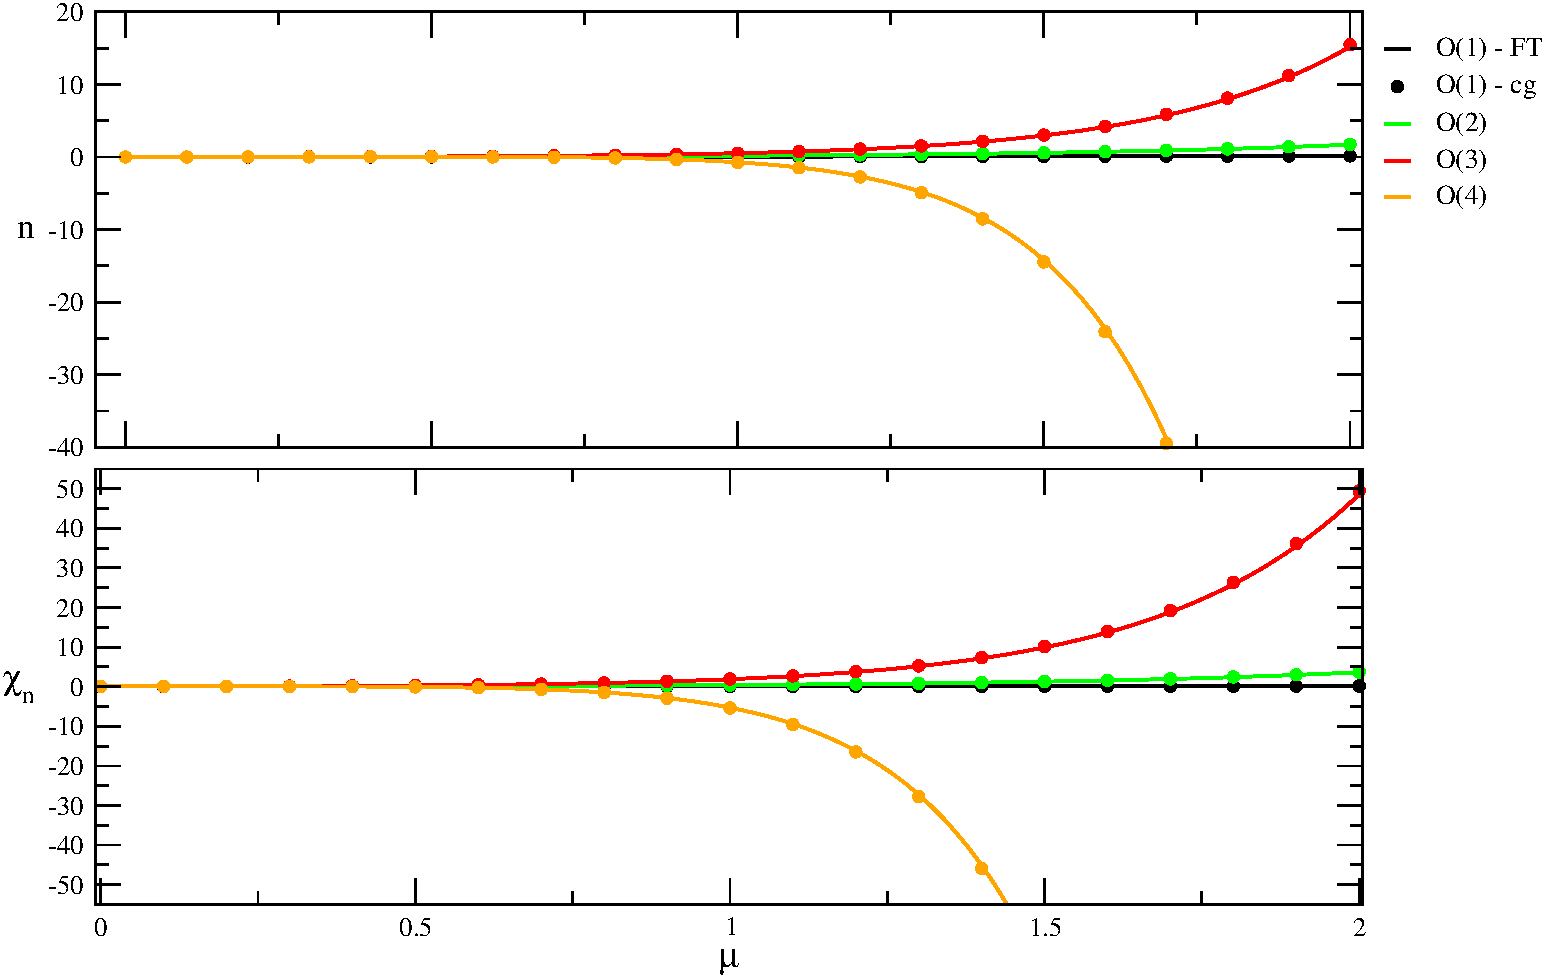
\includegraphics[width=0.84\textwidth,clip]{./mu_free}
\end{figure*}


\end{document}